\chapter[Le projet Aikon]{Le projet Aikon}

\section{Le contexte et les objectifs du projet Aikon}

\lettrine{A}{ikon est} une plateforme modulaire et open-source de vision par ordinateur, spécifiquement conçue pour les historiennes, les historiens et les chercheurs en humanités numériques. Son objectif principal est de mettre des algorithmes d'intelligence artificielle à la disposition d'utilisateurs ne possédant pas d'expertise technique en informatique. 


\subsection{Les objectifs scientifiques de la plateforme}
Les problématiques directement au coeur de la plateforme et de son utilisation sont : 

\begin{description}
\item[Comment mettre à disposition ces modèles aux chercheurs en SHS ?] Aikon n'est pas un projet de recherche lié à un sujet historique en particulier, c'est au contraire un projet fédérateur autour d'enjeux d'apport de la technique dans la méthode et donc un travail autant lié aux questions d'applicabilité des technologies d'intelligence artificielle que de l'évolution de l'historiographie au contacte des nouvelles méthodes informatiques. 

L'objectif de service de la plateforme est de permettre aux chercheurs de pratiquer une lecture distante\footnote{T. Arnold and L. Tilton, \og Distant Viewing: Analyzing Large Visual Corpora.\fg dans \textit{Digital Scholarship in the Humanities}, 2019} (\textit{distant viewing}) sur des corpus visuels massifs. Cette démarche s'appuie sur le traitement en masse pour transformer des documents en données exploitables. Aikon propose de récupéré de manière automatique des éléments structurants des documents comme les illustrations et d'y rechercher des régularités, des similarités. les visualisations globales (graphes, cartographies, représentations de similarité) permettent de faire émerger des tendances suspectées à l'œil humain à l'échelle d'un corpus entier, afin d'orienter le chercheur vers des cas d'études précis à analyser en détail.

\item[Comment obtenir des annotations expertes en pour affiner leurs prédictions ?] AIKON développe un paradigme interactif de \og l'humain dans la boucle \fg   (\textit{Human-in-the-loop}). L'approche \textit{HITL} offre une réduction de la pénibilité du travail d'annotation car la correction d'erreurs pré-existantes est nettement plus rapide et moins épuisante que le détourage manuel de milliers d'éléments visuels tout en résolvant le problème du manque de données de qualité annotées. De plus cette approche garantit à l'équipe d'Aikon et équipes de chercheurs un contrôle total sur les données qui servent à entraîner les outils d'analyse. La plateforme est développée selon les besoins des utilisateurs et attire des publics travaillant sur des sources très différentes. Le fait d'avoir autant de spécialistes de documents rares et difficiles, versant leurs fonds sur Aikon pour les étudier ouvre la voie à la constitution de datasets historiques précieux. L'un des objectifs scientifique d'Aikon et l'un des objectifs de notre stage est de réadapté des données d'annotation de documents en corpus d'entraînement pour de nouveaux modèles plus performants.
\end{description}

\begin{figure}[h]
    \centering
    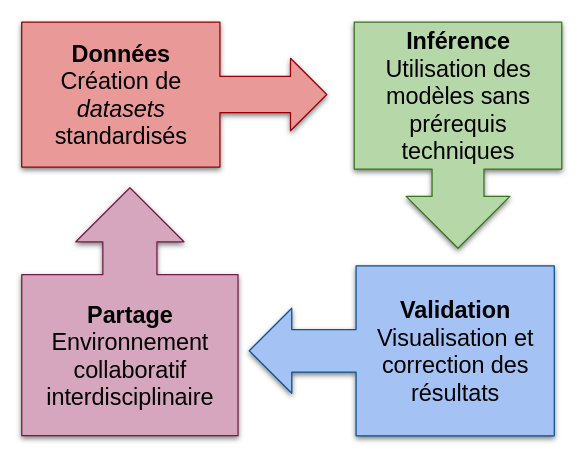
\includegraphics[scale=0.5]{img/aikonmethod.png}
    \caption{Le paradigme \textit{Human in the Loop} dans le projet Aikon}
    \label{fig:HITL}
\end{figure}

\subsection{Les réalisations techniques du projet}

Pour réussir ses missions, le méthodologie de l'équipe d'Aikon est de mettre en place un environnement perdurant sur long terme, étant capable de produire ses propres données d'entraînement avec l'aide de sa communauté de recherche et d'utilisateurs. 

Voici actuellement les fonctionnalités présentes sur les différentes instances de l'application d'Aikon\footnote{Informations tirées de la \href{https://docs.google.com/presentation/d/e/2PACX-1vTZ1cwAzy9YppXFgB3q9P-BXkFGck8F0FzdvrlTMDxhRdHxaPhinTWAIKyT_GATYEAgWEEE1mXrQvDt/pub?start=false&loop=false&delayms=3000\#slide=id.g306b6d3dc05_0_273}{présentation Aikon}} : 

\begin{description}
    \item \textbf{Documenter des sources historiques :} 
    Aikon offre une interface et un modèle de données conçu pour l'étude du lien intellectuel entre les sources. 
    
    \item \textbf{Gérer les numérisations des chercheurs:}
    Ensuite, les chercheurs peuvent importer leurs propres bases de données (images JPEG, PDF, IIIF \dots). La plateforme s'appuie sur le standard de référence IIIF (\textit{International Image Interoperability Framework}) pour gérer les images et les annotations, garantissant une forte interopérabilité avec les systèmes des bibliothèques et des archives. En s'appuyant sur les manifestes pour la gestion des images et des annotations, la plateforme s'insère de manière fluide dans n'importe quelle chaîne de traitement patrimoniale respectant ce standard comme par exemple \textit{Aikoncli}, un CLI développé durant le stage pour récupérer les annotations au format Yolo à partir d'un manifeste IIIF Aikon.  
    
    \item \textbf{Créer des corpus cohérents pour des traitements groupés :}
    Aikon offre une interface de gestion de la page à l'échelle du corpus de documents. 
    
    \item \textbf{Le traitement automatique des sources :} L'interface permet d'exécuter des tâches d'inférence sur les documents pour des analyses variées, comme l'extraction d'illustrations, de filigranes, la recherche de similarités visuelles entre plusieurs images, le regroupement (clustering) ou encore la vectorisation des diagrammes mathématiques.

    \item \textbf{La validation et la correction des résultats :} La plateforme est pensée pour l'interaction humaine. Les chercheurs peuvent annoter les documents et corriger les prédictions des modèles. Cela permet non seulement d'affiner leurs recherches, mais aussi de produire des données d'entraînement de qualité (vérité de terrain) qui pourront être réutilisées par les informaticiens pour améliorer les algorithmes.
\end{description}

Le projet est en cours de développement et d'amélioration actif avec notamment la détection des lignes et des régions d'écritures, du traitement des écritures (OCR/HTR), de la détection multiclasse\dots

\section{Les projets de recherche en vision artificielle historique}

Actuellement, la majorité des projets utilisant Aikon sont des consortiums de recherche en histoire des sciences. 

\subsection{Le projet Aikon et ses collaborateurs}


\begin{description}

\item[IMAGINE :] Imagine est un groupe de recherche hébergé à l'École Nationale des Ponts et Chaussées (ENPC, rattachée à l'Institut Polytechnique de Paris). Situé près de Paris, il fait partie de l'équipe A3SI au sein du laboratoire d'informatique Gaspard-Monge (LIGM). Les domaines de recherche d'Imagine sont la vision artificielle et l'apprentissage automatique\footnote{Site institutionnel d'\href{https://imagine-lab.enpc.fr/}{Imagine}}.

\begin{description}
    \item \textbf{ERC DISCOVER :} Porté par Mathieu Aubry au sein du laboratoire LIGM, Discover\footnote{Site institutionnel de \href{https://erc-discover.github.io/}{Discover}} est un projet de recherche fondamental financé par le Conseil Européen de la Recherche (bourse ERC Consolidator Grant). Le but est de développer la recherche en vision artificielle sur les \textit{structures visuelles} dans les domaines de la vision artificielle appliquées aux documents historiques et dans le domaine de l'imagerie terrestre. 
    
    Le projet Aikon est financé par Discover sous l'impulsion de Mathieu Aubry et Ségolène Albouy. L'objectif est de prouver que l'état de l'art de la vision artificielle peut être directement manipulé par des historiennes et des historiens sans prérequis en programmation informatique. L'une des grandes spécialités de l'équipe réside dans l'analyse de la similarité visuelle et la correspondance de motifs complexes. Dans l'application Aikon, cette expertise se traduit par des fonctionnalités de clustering et de recherche d'images par le contenu. Les informaticien\pmm nes d'IMAGINE travaillent également à de meilleurs algorithmes d'OCR et d'HTR à intégrer dans Aikon. 
\end{description}

\item[EIDA :]

\textit{Editing and Analysing hIstorical astronomical Diagrams with Artificial intelligence} est un projet coordoné par l'historien Matthieu Husson, lié à l'Observatoire de Paris et financé par l'Agence nationale de la recherche. C'est un programme d'étude d'histoire de l'astronomie à l'aide de technologies de vision artificielle en lien avec les autres activités de Matthieu Husson d'analyse des sources anciennes (notamment à travers la conception du système d'information DISHAS et la direction du projet européen ERC ALFA)

EIDA s'attaque au langage visuel et géométrique de la science. L'objectif est de détecter, d'extraire, de classifier et de comparer automatiquement les diagrammes astronomiques. L'enjeu historique est de comprendre comment le savoir scientifique (modèles cosmologiques, calculs d'éclipses, mouvements planétaires) a circulé, été copié et modifié à travers l'Europe et le bassin méditerranéen.

Le projet se concentre sur les manuscrits médiévaux et les premiers incunables (traités d'astronomie, tables astronomiques, commentaires de la Sphère de Sacrobosco). Ces documents sont particulièrement complexes car le texte s'enroule souvent autour des diagrammes, et les figures géométriques varient énormément selon la main du copiste.

L'une des spécificités du projet est l'étude des tables astronomiques. L'étude des données tabulaires est l'un des sujets qui a été le plus difficile au sein de la création du corpus GenHisDoc dont l'un des objectifs était de réussir à détecter les tables dans les documents historiques. 

\item[Le projet VHS :] \textit{Vision and Historical analysis of Scientific illustration circulation} est coordoné par l'historien des mathématique Alexandre Guilbaud et supporté par Sorbonne Université et l'Agence nationale de Recherche. C'est un projet au croisement de l'histoire de l'art, de l'histoire des sciences et des humanités numériques. Il s'agit d'un programme interdisciplinaire associant plusieurs institutions, notamment Sorbonne Université (via l'Institut des sciences du calcul et des données --- ISCD, et le laboratoire LIP6), le CNRS (Orient \& Méditerranée) et l'équipe IMAGINE de l'École des Ponts ParisTech.

Le but scientifique de VHS est d'appliquer les méthodes d'apprentissage profond (Deep Learning) pour analyser la circulation et la réutilisation des images dans l'histoire scientifique ou culturelle. Il s'agit de repérer des motifs récurrents, de tracer l'évolution d'une iconographie au fil des siècles, et de constituer des stemmata grâce à l'étude a similarité visuelle entre les illustrations. L'ambition centrale du projet VHS est de renouveler l'approche historique de la circulation des savoirs scientifiques en se focalisant non plus sur le texte, mais sur l'image et la pensée visuelle.  

Les corpus sont souvent plus hétérogènes que ceux d'EIDA. Ils englobent des imprimés richement illustrés, des estampes, des planches anatomiques ou botaniques, et des schémas techniques. L'enjeu pour le modèle de vision n'est pas seulement de détecter \og où \fg~est l'image (détection d'objet), mais de comprendre \og de quoi \fg~elle est proche visuellement dans le reste du corpus.


\end{description}

\subsection{Les autres projets de vision artificielle historique :}

Parmi les projets de recherche appliquant la vision artificielle à l'histoire et aux humanités numériques, certains sont dotés de plateformes en ligne qui proposent à l’utilisateur d’explorer leurs corpus visuels et de découvrir leurs travaux. Dans la conception de l’application du projet AIkon et de la capacité des modèles à entrainer, il est essentiel de proposer des fonctionnalités d’analyse et d'exploration visuelle qui viennent compléter les outils existants. Dans cette mesure, l’examen des dispositifs de recherche par l'image et de détection actuels, tout comme l'identification de leurs limites, s'avère éclairant pour cibler les besoins des utilisateurs dans le cadre d’un projet collaboratif, tout en prenant en compte la diversité des approches face aux sources iconographiques.


\begin{description}
    
        \item[Le Consortium Pictoria :] Le \textit{Programme d'Identification, Classification, Traitement d'Images, Observation et Reconnaissance des formes par l'Intelligence Artificielle}\footnote{Site institutionnel de  \href{https://pictoria.hypotheses.org/}{Pictoria}} est un consortium-HN supporté par la Maison des Sciences Humaines et Sociales Mondes et coordonné par Julien Schuh. Cette initiative fédère la recherche interdisciplinaire autour de la reconnaissance automatique de formes appliquée aux sciences humaines et sociales. Son action vise à faciliter l'accès, l'interconnexion et l'enrichissement des corpus visuels (histoire de l'art, archéologie, histoire de l'architecture, sociologie, etc.) en développant des protocoles partagés, des formations, des tutoriels ainsi que des prototypes applicatifs.

        Porté par une dynamique nationale et internationale, le projet réunit des laboratoires de recherche ainsi que des institutions patrimoniales de premier plan, parmi lesquelles la BnF, l’INHA, l’INA, l’École nationale des chartes ou encore La contemporaine ...

        Pictoria met à disposition des notebooks jupyter de tutoriels pour les chercheurs ainsi que des listes d'outils sur SSH Open Market Place et contribue à faire conna\^itre le projet Aikon. 
        
        \item[Gallica :] 
        
        La BnF propose ou a proposé plusieurs projets liés à la vision artificielle historique notamment par le travail de Jean-Philippe Moreux. 
        
        --- La BnF propose par sur son site BnF Api\footnote{Lien vers le \href{https://api.bnf.fr/fr/node/181\#scroll-nav\_\_1}{site institutionnel de l'api BnF}} des collections de jeu de données d'images annotés pour la classification.
        
        --- GallicaPix, un démonstrateur qui n'est plus en ligne aujourd'hui, de recherche visuelle de détection et de segmentation des images (cartes, gravures, photographies) 
        
        Nous avions étudié le fait de réutiliser des jeux de données Gallica, la complexité de réutilisation des formats d'annotations dans un temps très court nous à amener à envisager d'autres jeux de données. 
        
        \item[Arkindex / Teklia :] Développée par une entreprise française cette plateforme couple HTR, classification de page, détection et segmentation. Arkindex est notamment utilisé par le projet SocFace réunissant l'Institut national d'études démographiques (INED), les Archives nationales et Teklia. 
        
        Le dataset Horae de l'IRHT publié sur Zenodo a notamment été produit en utilisant Arkindex et des modèles entraînés sur Horae peuvent y être testé.  Contrairement à l'application Aikon actuelle, Arkindex peut travailler avec du texte imprimé et manuscrit et donc les données qui en sortent sont bien plus complexes qu'un simple dataset de détection. Nous avons donc étudier l'ontologie d'annotation d'Horae directement sur Arkindex avant de télécharger et modifier le dataset pour nos propres besoins.
        
        De la même manière que AIkon, Arkindex permet de déployer plusieurs modèles différents sur la même plateforme pour plusieurs types de tâches et d'utiliser cette méthode d'\textit{Human in the loop} pour pré-annoter et corriger des corpus. 
        
        \item[Newspaper Navigator / Library of Congress, USA :] Issue du projet \textit{Chronicling America}\footnote{Site institutionnel du \href{https://labs.loc.gov/work/experiments/newspaper-navigator/}{projet Newspaper Navigator}} et mené par Benjamin Lee. Ce projet s'appuie sur la détection d'objets pour extraire et indexer des millions de photographies, cartes, dessins et publicités dans les archives de la presse américaine.
        
        Nous sommes allés assez loin dans la réutilisation des annotations de Newspaper Navigator, jusqu'au point que de la correction et de l'incorporation du dataset. Newspaper Navigator était notamment intéressant pour la quantité de photographies et dessins contemporains à l'intérieur, le transfert d'une ontologie d'annotation à une autre était difficile. Nous avons donc retiré tout le corpus de presse avant la phase d'entraînement et d'évaluation des modèles de test.
        
        \item[Machines Reading Maps / Alan Turing Institute :] Un outil d'analyse visuelle\footnote{Site institutionnel du projet \href{https://www.turing.ac.uk/research/research-projects/machines-reading-maps}{Machines Reading Maps}.} permettant aux chercheurs de fouiller des cartes historiques à grande échelle pour y détecter automatiquement des bâtiments, des voies ferrées ou des particularités topographiques.
        
        La question de détecter les cartes au sein du dataset GenHisDoc a été une idée rapidement abandonnée car nous avons considéré qu'une carte au sein d'un texte serait plus simplement détectée comme une illustration et sans réel besoin d'annotation sur mesure. 
        
        \item [dhSegment / Digital Humanities Laboratory :] Développé originalement par Benoit Seguin et Sofia Ares Oliveira. dhSegment est une architecture de deep learning spécifiquement développée pour la segmentation des documents historiques complexes, allant de l'extraction de lignes à la détection de bordures et d'illustrations.
        
        Nous nous sommes rapidement orienté vers une approche de détection d'éléments plutôt que de segmentation. Cependant la dhSegment a été l'une des sources envisagée pour la création de masques de segmentation ou la conversion masque de segmentation vers boîtes englobantes. 

        \item[TORNE-H / École nationale des chartes \& Musée des arts décoratifs :] Coordoné par Mme Emmanuelle Bermès, le projet Torne-H développe des outils et des méthodes d'utilisation du machine learning dans le monde muséal et archivistique. L'application TiamaT (\textit{Toolkit for Integrated Annotation and Machine-learning Assisted Training}), développée par Marion Charpier et Fantin Le Ber s'attaque comme Aikon à la question de la préannotation des données pour l'entrainement de modèles avec le m\^eme paradigme d'amélioration itérative \textit{Human in the Loop}\footnote{Présentation de TiamaT sur \href{https://marketplace.sshopencloud.eu/tool-or-service/lYN2OC}{SSHopen Marketplace}}.
        
\end{description}